\section{Results}
\label{sec:results}

We first present the main long-term forecasting comparison across seven datasets
against eight baselines including two recent ICLR Transformer models, then
analyze distribution-shift robustness and non-stationary regimes. All accuracy
numbers are test MSE and MAE in the train-standardized space, averaged over
horizon steps and channels, reported as mean $\pm$ std over three seeds; the
best result in each row is in bold and the second best underlined.

\subsection{Main Comparison}
\label{sec:results:main}

Tables~\ref{tab:main_L336} and~\ref{tab:main_L96} report the headline
comparisons at $L{=}336$ and $L{=}96$ on the five standard benchmarks;
Table~\ref{tab:main_L336_large} extends the $L{=}336$ comparison to the
two high-variate datasets (Electricity and Traffic).

\IfFileExists{../results/tables/main_table_L336.tex}{%
  \begingroup\fitwidetables% Auto-generated by scripts/make_tables.py — do not edit by hand.
\begin{table*}[t]
\centering
\setlength{\tabcolsep}{3pt}
\caption{Long-term forecasting results (lookback $L=336$). Each cell is test MSE/MAE (mean$\pm$std over 3 seeds) in the train-standardized space. \textbf{Bold}: best; \underline{{underline}}: second best. Standard benchmarks. PatchTST* uses a 4\,GB-feasible small config.}
\label{tab:main_L336}
\begin{tabular}{llcccccccccccccccccc}
\toprule
Dataset & $H$ & \multicolumn{2}{c}{Naive} & \multicolumn{2}{c}{NLinear} & \multicolumn{2}{c}{DLinear} & \multicolumn{2}{c}{RLinear} & \multicolumn{2}{c}{FITS} & \multicolumn{2}{c}{PatchTST*} & \multicolumn{2}{c}{iTransformer} & \multicolumn{2}{c}{TimesNet} & \multicolumn{2}{c}{FreqLite} \\
\cmidrule(lr){3-4} \cmidrule(lr){5-6} \cmidrule(lr){7-8} \cmidrule(lr){9-10} \cmidrule(lr){11-12} \cmidrule(lr){13-14} \cmidrule(lr){15-16} \cmidrule(lr){17-18} \cmidrule(lr){19-20}
& & MSE & MAE & MSE & MAE & MSE & MAE & MSE & MAE & MSE & MAE & MSE & MAE & MSE & MAE & MSE & MAE & MSE & MAE \\
\midrule
ETTh1 & 96 & 1.294\textpm0.000 & 0.713\textpm0.000 & 0.384\textpm0.005 & 0.405\textpm0.004 & \underline{0.376\textpm0.001} & \underline{0.398\textpm0.002} & 0.379\textpm0.003 & 0.400\textpm0.003 & 0.399\textpm0.000 & 0.419\textpm0.000 & 0.431\textpm0.043 & 0.434\textpm0.024 & 0.403\textpm0.002 & 0.416\textpm0.002 & 0.457\textpm0.051 & 0.454\textpm0.020 & \textbf{0.373\textpm0.001} & \textbf{0.395\textpm0.001} \\
 & 192 & 1.325\textpm0.000 & 0.733\textpm0.000 & 0.413\textpm0.001 & 0.421\textpm0.000 & 0.418\textpm0.009 & 0.428\textpm0.009 & \underline{0.412\textpm0.001} & \underline{0.419\textpm0.001} & 0.429\textpm0.000 & 0.436\textpm0.000 & 0.444\textpm0.006 & 0.445\textpm0.005 & 0.447\textpm0.010 & 0.445\textpm0.007 & 0.530\textpm0.035 & 0.499\textpm0.017 & \textbf{0.410\textpm0.005} & \textbf{0.417\textpm0.005} \\
 & 336 & 1.330\textpm0.000 & 0.746\textpm0.000 & \underline{0.438\textpm0.002} & \underline{0.437\textpm0.002} & 0.453\textpm0.011 & 0.454\textpm0.011 & 0.442\textpm0.007 & 0.440\textpm0.006 & 0.451\textpm0.000 & 0.448\textpm0.000 & 0.552\textpm0.058 & 0.503\textpm0.027 & 0.472\textpm0.017 & 0.461\textpm0.010 & 0.600\textpm0.106 & 0.539\textpm0.047 & \textbf{0.432\textpm0.001} & \textbf{0.430\textpm0.001} \\
 & 720 & 1.335\textpm0.000 & 0.755\textpm0.000 & \underline{0.444\textpm0.000} & \underline{0.459\textpm0.000} & 0.488\textpm0.016 & 0.501\textpm0.012 & 0.449\textpm0.002 & 0.463\textpm0.002 & 0.447\textpm0.001 & 0.466\textpm0.001 & 0.630\textpm0.029 & 0.557\textpm0.014 & 0.485\textpm0.011 & 0.489\textpm0.007 & 0.673\textpm0.031 & 0.577\textpm0.015 & \textbf{0.444\textpm0.002} & \textbf{0.459\textpm0.002} \\
\midrule
ETTh2 & 96 & 0.432\textpm0.000 & 0.422\textpm0.000 & 0.283\textpm0.001 & 0.344\textpm0.001 & 0.285\textpm0.003 & 0.350\textpm0.003 & \underline{0.281\textpm0.000} & \underline{0.342\textpm0.000} & 0.285\textpm0.001 & 0.346\textpm0.000 & 0.346\textpm0.016 & 0.382\textpm0.008 & 0.322\textpm0.015 & 0.371\textpm0.006 & 0.406\textpm0.024 & 0.427\textpm0.007 & \textbf{0.275\textpm0.001} & \textbf{0.336\textpm0.000} \\
 & 192 & 0.534\textpm0.000 & 0.473\textpm0.000 & 0.347\textpm0.003 & 0.386\textpm0.001 & 0.385\textpm0.009 & 0.420\textpm0.005 & 0.349\textpm0.013 & 0.386\textpm0.006 & \underline{0.344\textpm0.000} & \underline{0.383\textpm0.000} & 0.423\textpm0.029 & 0.429\textpm0.013 & 0.401\textpm0.018 & 0.418\textpm0.009 & 0.425\textpm0.023 & 0.441\textpm0.010 & \textbf{0.340\textpm0.005} & \textbf{0.380\textpm0.003} \\
 & 336 & 0.597\textpm0.000 & 0.511\textpm0.000 & 0.384\textpm0.013 & 0.415\textpm0.006 & 0.457\textpm0.007 & 0.469\textpm0.005 & 0.369\textpm0.004 & 0.407\textpm0.002 & \underline{0.364\textpm0.000} & \textbf{0.401\textpm0.000} & 0.432\textpm0.006 & 0.440\textpm0.003 & 0.410\textpm0.003 & 0.430\textpm0.001 & 0.431\textpm0.015 & 0.447\textpm0.012 & \textbf{0.362\textpm0.001} & \underline{0.402\textpm0.000} \\
 & 720 & 0.594\textpm0.000 & 0.519\textpm0.000 & 0.407\textpm0.007 & 0.442\textpm0.002 & 0.701\textpm0.027 & 0.594\textpm0.012 & 0.397\textpm0.001 & 0.433\textpm0.000 & \textbf{0.391\textpm0.000} & \textbf{0.427\textpm0.000} & 0.421\textpm0.016 & 0.447\textpm0.008 & 0.441\textpm0.005 & 0.458\textpm0.001 & 0.479\textpm0.006 & 0.481\textpm0.001 & \underline{0.392\textpm0.002} & \underline{0.430\textpm0.001} \\
\midrule
ETTm1 & 96 & 1.214\textpm0.000 & 0.665\textpm0.000 & 0.305\textpm0.002 & 0.347\textpm0.002 & \textbf{0.300\textpm0.001} & \underline{0.344\textpm0.000} & 0.305\textpm0.004 & 0.346\textpm0.003 & 0.304\textpm0.000 & 0.346\textpm0.000 & 0.302\textpm0.013 & 0.352\textpm0.008 & 0.323\textpm0.010 & 0.364\textpm0.001 & 0.380\textpm0.029 & 0.397\textpm0.013 & \underline{0.302\textpm0.001} & \textbf{0.344\textpm0.001} \\
 & 192 & 1.261\textpm0.000 & 0.690\textpm0.000 & 0.343\textpm0.003 & 0.370\textpm0.003 & \textbf{0.337\textpm0.002} & 0.368\textpm0.003 & 0.338\textpm0.003 & \underline{0.366\textpm0.003} & \underline{0.338\textpm0.000} & \textbf{0.366\textpm0.000} & 0.345\textpm0.001 & 0.381\textpm0.003 & 0.356\textpm0.007 & 0.385\textpm0.003 & 0.472\textpm0.040 & 0.441\textpm0.021 & 0.340\textpm0.004 & 0.367\textpm0.003 \\
 & 336 & 1.287\textpm0.000 & 0.707\textpm0.000 & 0.374\textpm0.002 & 0.386\textpm0.001 & \textbf{0.372\textpm0.001} & 0.390\textpm0.001 & 0.373\textpm0.001 & 0.386\textpm0.001 & 0.372\textpm0.000 & \underline{0.385\textpm0.000} & 0.381\textpm0.011 & 0.401\textpm0.006 & 0.385\textpm0.005 & 0.405\textpm0.002 & 0.454\textpm0.007 & 0.443\textpm0.002 & \underline{0.372\textpm0.001} & \textbf{0.384\textpm0.001} \\
 & 720 & 1.322\textpm0.000 & 0.729\textpm0.000 & 0.431\textpm0.003 & 0.419\textpm0.002 & \underline{0.428\textpm0.004} & 0.424\textpm0.006 & 0.431\textpm0.003 & 0.418\textpm0.001 & \textbf{0.428\textpm0.000} & \textbf{0.416\textpm0.000} & 0.429\textpm0.007 & 0.436\textpm0.006 & 0.441\textpm0.002 & 0.435\textpm0.002 & 0.520\textpm0.044 & 0.478\textpm0.015 & 0.428\textpm0.001 & \underline{0.417\textpm0.001} \\
\midrule
ETTm2 & 96 & 0.266\textpm0.000 & 0.328\textpm0.000 & 0.167\textpm0.001 & 0.257\textpm0.000 & 0.169\textpm0.002 & 0.265\textpm0.002 & \underline{0.166\textpm0.000} & \underline{0.255\textpm0.000} & 0.167\textpm0.000 & 0.256\textpm0.000 & 0.177\textpm0.002 & 0.262\textpm0.001 & 0.187\textpm0.005 & 0.275\textpm0.005 & 0.201\textpm0.004 & 0.280\textpm0.003 & \textbf{0.164\textpm0.001} & \textbf{0.253\textpm0.000} \\
 & 192 & 0.340\textpm0.000 & 0.371\textpm0.000 & 0.222\textpm0.000 & 0.294\textpm0.000 & 0.229\textpm0.006 & 0.308\textpm0.009 & \underline{0.221\textpm0.000} & \underline{0.292\textpm0.000} & 0.222\textpm0.000 & 0.293\textpm0.000 & 0.243\textpm0.009 & 0.308\textpm0.005 & 0.250\textpm0.009 & 0.317\textpm0.006 & 0.267\textpm0.011 & 0.325\textpm0.007 & \textbf{0.219\textpm0.000} & \textbf{0.290\textpm0.000} \\
 & 336 & 0.412\textpm0.000 & 0.410\textpm0.000 & 0.276\textpm0.000 & 0.329\textpm0.000 & 0.304\textpm0.023 & 0.362\textpm0.022 & \underline{0.275\textpm0.000} & 0.327\textpm0.000 & 0.275\textpm0.000 & \underline{0.327\textpm0.000} & 0.310\textpm0.009 & 0.350\textpm0.006 & 0.302\textpm0.008 & 0.349\textpm0.004 & 0.309\textpm0.017 & 0.350\textpm0.010 & \textbf{0.274\textpm0.001} & \textbf{0.326\textpm0.000} \\
 & 720 & 0.522\textpm0.000 & 0.466\textpm0.000 & 0.371\textpm0.000 & 0.386\textpm0.000 & 0.431\textpm0.017 & 0.443\textpm0.010 & \underline{0.369\textpm0.000} & 0.384\textpm0.000 & \textbf{0.368\textpm0.000} & \textbf{0.383\textpm0.000} & 0.387\textpm0.007 & 0.403\textpm0.007 & 0.396\textpm0.006 & 0.406\textpm0.005 & 0.428\textpm0.028 & 0.418\textpm0.015 & 0.370\textpm0.004 & \underline{0.383\textpm0.001} \\
\midrule
Weather & 96 & 0.259\textpm0.000 & 0.254\textpm0.000 & 0.174\textpm0.001 & 0.224\textpm0.002 & 0.174\textpm0.000 & 0.235\textpm0.001 & 0.175\textpm0.001 & 0.224\textpm0.001 & 0.176\textpm0.000 & 0.228\textpm0.000 & \textbf{0.149\textpm0.001} & \textbf{0.197\textpm0.001} & \underline{0.160\textpm0.002} & \underline{0.210\textpm0.001} & 0.183\textpm0.015 & 0.235\textpm0.012 & 0.174\textpm0.000 & 0.224\textpm0.001 \\
 & 192 & 0.309\textpm0.000 & 0.292\textpm0.000 & 0.217\textpm0.000 & 0.260\textpm0.000 & 0.217\textpm0.001 & 0.275\textpm0.002 & 0.218\textpm0.000 & 0.260\textpm0.000 & 0.219\textpm0.000 & 0.263\textpm0.000 & \textbf{0.195\textpm0.002} & \textbf{0.241\textpm0.001} & \underline{0.206\textpm0.000} & \underline{0.252\textpm0.001} & 0.250\textpm0.028 & 0.289\textpm0.019 & 0.218\textpm0.000 & 0.260\textpm0.001 \\
 & 336 & 0.376\textpm0.000 & 0.338\textpm0.000 & 0.266\textpm0.000 & 0.296\textpm0.000 & 0.262\textpm0.001 & 0.313\textpm0.003 & 0.265\textpm0.000 & 0.295\textpm0.000 & 0.267\textpm0.000 & 0.297\textpm0.000 & \textbf{0.248\textpm0.002} & \textbf{0.283\textpm0.004} & \underline{0.256\textpm0.002} & \underline{0.289\textpm0.000} & 0.332\textpm0.003 & 0.341\textpm0.003 & 0.265\textpm0.000 & 0.295\textpm0.000 \\
 & 720 & 0.465\textpm0.000 & 0.394\textpm0.000 & 0.334\textpm0.000 & 0.344\textpm0.000 & 0.333\textpm0.007 & 0.376\textpm0.009 & 0.333\textpm0.000 & 0.342\textpm0.000 & 0.334\textpm0.000 & 0.343\textpm0.000 & \underline{0.329\textpm0.008} & \underline{0.339\textpm0.006} & \textbf{0.327\textpm0.003} & \textbf{0.339\textpm0.002} & 0.400\textpm0.007 & 0.387\textpm0.004 & 0.333\textpm0.000 & 0.342\textpm0.000 \\
\bottomrule
\end{tabular}
\end{table*}
\endgroup%
}{\begin{table*}[t]\centering\caption{Main results at $L{=}336$ (standard benchmarks).}%
  \label{tab:main_L336}\textit{[main results table at $L{=}336$ pending]}\end{table*}}

\IfFileExists{../results/tables/main_table_L336_large.tex}{%
  \begingroup\fitwidetables% Auto-generated by scripts/make_tables.py — do not edit by hand.
\begin{table*}[t]
\centering
\setlength{\tabcolsep}{3pt}
\caption{Long-term forecasting results (lookback $L=336$). Each cell is test MSE/MAE (mean$\pm$std over 3 seeds) in the train-standardized space. \textbf{Bold}: best; \underline{{underline}}: second best. Electricity ($C{=}321$) and Traffic ($C{=}862$). PatchTST* omitted (4\,GB-infeasible at these channel counts).}
\label{tab:main_L336_large}
\begin{tabular}{llcccccccccccccccccc}
\toprule
Dataset & $H$ & \multicolumn{2}{c}{Naive} & \multicolumn{2}{c}{NLinear} & \multicolumn{2}{c}{DLinear} & \multicolumn{2}{c}{RLinear} & \multicolumn{2}{c}{FITS} & \multicolumn{2}{c}{PatchTST*} & \multicolumn{2}{c}{iTransformer} & \multicolumn{2}{c}{TimesNet} & \multicolumn{2}{c}{FreqLite} \\
\cmidrule(lr){3-4} \cmidrule(lr){5-6} \cmidrule(lr){7-8} \cmidrule(lr){9-10} \cmidrule(lr){11-12} \cmidrule(lr){13-14} \cmidrule(lr){15-16} \cmidrule(lr){17-18} \cmidrule(lr){19-20}
& & MSE & MAE & MSE & MAE & MSE & MAE & MSE & MAE & MSE & MAE & MSE & MAE & MSE & MAE & MSE & MAE & MSE & MAE \\
\midrule
Electricity & 96 & 1.588\textpm0.000 & 0.945\textpm0.000 & 0.141\textpm0.000 & 0.237\textpm0.000 & \underline{0.140\textpm0.000} & 0.238\textpm0.000 & 0.141\textpm0.000 & 0.236\textpm0.000 & 0.188\textpm0.000 & 0.301\textpm0.000 & -- & -- & \textbf{0.134\textpm0.000} & \textbf{0.230\textpm0.000} & 0.191\textpm0.008 & 0.296\textpm0.007 & 0.140\textpm0.000 & \underline{0.235\textpm0.000} \\
 & 192 & 1.596\textpm0.000 & 0.951\textpm0.000 & 0.156\textpm0.000 & 0.250\textpm0.000 & \underline{0.154\textpm0.000} & 0.251\textpm0.000 & 0.155\textpm0.000 & \underline{0.248\textpm0.000} & 0.201\textpm0.000 & 0.310\textpm0.000 & -- & -- & \textbf{0.153\textpm0.000} & 0.248\textpm0.000 & 0.205\textpm0.004 & 0.306\textpm0.003 & 0.154\textpm0.000 & \textbf{0.247\textpm0.000} \\
 & 336 & 1.618\textpm0.000 & 0.961\textpm0.000 & 0.172\textpm0.000 & 0.266\textpm0.000 & \underline{0.170\textpm0.000} & 0.268\textpm0.000 & 0.172\textpm0.000 & 0.265\textpm0.000 & 0.216\textpm0.000 & 0.323\textpm0.000 & -- & -- & \textbf{0.169\textpm0.001} & \underline{0.264\textpm0.001} & 0.207\textpm0.000 & 0.311\textpm0.001 & 0.171\textpm0.000 & \textbf{0.264\textpm0.000} \\
 & 720 & 1.647\textpm0.000 & 0.975\textpm0.000 & 0.211\textpm0.000 & 0.299\textpm0.000 & \textbf{0.204\textpm0.000} & 0.301\textpm0.000 & 0.210\textpm0.000 & \underline{0.297\textpm0.000} & 0.252\textpm0.000 & 0.349\textpm0.000 & -- & -- & \underline{0.208\textpm0.002} & 0.298\textpm0.003 & 0.231\textpm0.001 & 0.327\textpm0.004 & 0.210\textpm0.000 & \textbf{0.296\textpm0.000} \\
\midrule
Traffic & 96 & 2.714\textpm0.000 & 1.077\textpm0.000 & 0.411\textpm0.000 & 0.281\textpm0.000 & 0.410\textpm0.000 & 0.283\textpm0.000 & 0.410\textpm0.000 & 0.279\textpm0.000 & 0.520\textpm0.000 & 0.385\textpm0.000 & -- & -- & \textbf{0.381\textpm0.002} & \textbf{0.275\textpm0.000} & 0.611\textpm0.010 & 0.331\textpm0.004 & \underline{0.410\textpm0.000} & \underline{0.278\textpm0.000} \\
 & 192 & 2.747\textpm0.000 & 1.085\textpm0.000 & 0.424\textpm0.000 & 0.286\textpm0.000 & 0.423\textpm0.000 & 0.288\textpm0.000 & 0.423\textpm0.000 & \underline{0.283\textpm0.000} & 0.532\textpm0.000 & 0.389\textpm0.000 & -- & -- & \textbf{0.406\textpm0.000} & 0.288\textpm0.000 & 0.632\textpm0.015 & 0.341\textpm0.008 & \underline{0.423\textpm0.000} & \textbf{0.283\textpm0.000} \\
 & 336 & 2.788\textpm0.000 & 1.094\textpm0.000 & 0.437\textpm0.000 & 0.293\textpm0.000 & 0.436\textpm0.000 & 0.296\textpm0.000 & 0.436\textpm0.000 & \underline{0.290\textpm0.000} & 0.543\textpm0.000 & 0.393\textpm0.000 & -- & -- & \textbf{0.421\textpm0.000} & 0.295\textpm0.000 & 0.634\textpm0.003 & 0.341\textpm0.004 & \underline{0.435\textpm0.000} & \textbf{0.289\textpm0.000} \\
 & 720 & 2.809\textpm0.000 & 1.097\textpm0.000 & 0.465\textpm0.000 & 0.310\textpm0.000 & 0.466\textpm0.000 & 0.315\textpm0.000 & 0.464\textpm0.000 & \underline{0.306\textpm0.000} & 0.564\textpm0.000 & 0.403\textpm0.000 & -- & -- & \textbf{0.450\textpm0.000} & 0.311\textpm0.000 & 0.667\textpm0.003 & 0.356\textpm0.002 & \underline{0.463\textpm0.000} & \textbf{0.306\textpm0.000} \\
\bottomrule
\end{tabular}
\end{table*}
\endgroup%
}{\begin{table*}[t]\centering\caption{Large-scale results at $L{=}336$.}%
  \label{tab:main_L336_large}\textit{[large-scale results table pending]}\end{table*}}

\IfFileExists{../results/tables/main_table_L96.tex}{%
  \begingroup\fitwidetables% Auto-generated by scripts/make_tables.py — do not edit by hand.
\begin{table*}[t]
\centering
\setlength{\tabcolsep}{3pt}
\caption{Long-term forecasting results (lookback $L=96$). Each cell is test MSE/MAE (mean$\pm$std over 3 seeds) in the train-standardized space. \textbf{Bold}: best; \underline{underline}: second best. PatchTST* uses a 4\,GB-feasible small config.}
\label{tab:main_L96}
\begin{tabular}{llcccccccccccccc}
\toprule
Dataset & $H$ & \multicolumn{2}{c}{Naive} & \multicolumn{2}{c}{NLinear} & \multicolumn{2}{c}{DLinear} & \multicolumn{2}{c}{RLinear} & \multicolumn{2}{c}{FITS} & \multicolumn{2}{c}{PatchTST*} & \multicolumn{2}{c}{FreqLite} \\
\cmidrule(lr){3-4} \cmidrule(lr){5-6} \cmidrule(lr){7-8} \cmidrule(lr){9-10} \cmidrule(lr){11-12} \cmidrule(lr){13-14} \cmidrule(lr){15-16}
& & MSE & MAE & MSE & MAE & MSE & MAE & MSE & MAE & MSE & MAE & MSE & MAE & MSE & MAE \\
\midrule
ETTh1 & 96 & 1.294\textpm0.000 & 0.713\textpm0.000 & 0.398\textpm0.003 & 0.407\textpm0.003 & 0.390\textpm0.003 & 0.404\textpm0.005 & 0.391\textpm0.000 & 0.399\textpm0.000 & 0.409\textpm0.001 & 0.417\textpm0.000 & \textbf{0.376\textpm0.003} & \underline{0.396\textpm0.000} & \underline{0.386\textpm0.000} & \textbf{0.394\textpm0.000} \\
 & 192 & 1.325\textpm0.000 & 0.733\textpm0.000 & 0.446\textpm0.001 & 0.433\textpm0.001 & \underline{0.440\textpm0.003} & 0.434\textpm0.004 & 0.443\textpm0.001 & \underline{0.429\textpm0.001} & 0.459\textpm0.001 & 0.446\textpm0.001 & 0.442\textpm0.000 & 0.436\textpm0.003 & \textbf{0.437\textpm0.000} & \textbf{0.423\textpm0.000} \\
 & 336 & 1.330\textpm0.000 & 0.746\textpm0.000 & 0.488\textpm0.001 & 0.454\textpm0.001 & 0.487\textpm0.004 & 0.464\textpm0.004 & \underline{0.486\textpm0.000} & \underline{0.450\textpm0.000} & 0.504\textpm0.005 & 0.470\textpm0.005 & 0.507\textpm0.003 & 0.469\textpm0.002 & \textbf{0.481\textpm0.000} & \textbf{0.446\textpm0.000} \\
 & 720 & 1.335\textpm0.000 & 0.755\textpm0.000 & \underline{0.482\textpm0.000} & \underline{0.472\textpm0.000} & 0.510\textpm0.002 & 0.505\textpm0.002 & 0.487\textpm0.000 & 0.474\textpm0.000 & 0.496\textpm0.007 & 0.488\textpm0.005 & 0.529\textpm0.022 & 0.500\textpm0.007 & \textbf{0.482\textpm0.000} & \textbf{0.470\textpm0.000} \\
\midrule
ETTh2 & 96 & 0.432\textpm0.000 & 0.422\textpm0.000 & 0.298\textpm0.000 & 0.347\textpm0.000 & 0.327\textpm0.002 & 0.382\textpm0.003 & \underline{0.295\textpm0.000} & \underline{0.344\textpm0.000} & 0.303\textpm0.000 & 0.349\textpm0.001 & 0.298\textpm0.007 & 0.346\textpm0.004 & \textbf{0.290\textpm0.000} & \textbf{0.339\textpm0.000} \\
 & 192 & 0.534\textpm0.000 & 0.473\textpm0.000 & 0.385\textpm0.000 & 0.399\textpm0.000 & 0.450\textpm0.005 & 0.457\textpm0.003 & 0.382\textpm0.000 & 0.396\textpm0.000 & 0.387\textpm0.001 & 0.398\textpm0.001 & \textbf{0.376\textpm0.006} & \underline{0.394\textpm0.004} & \underline{0.376\textpm0.000} & \textbf{0.391\textpm0.000} \\
 & 336 & 0.597\textpm0.000 & 0.511\textpm0.000 & 0.425\textpm0.001 & 0.434\textpm0.000 & 0.567\textpm0.010 & 0.527\textpm0.005 & \underline{0.421\textpm0.000} & \underline{0.431\textpm0.000} & 0.424\textpm0.001 & 0.432\textpm0.000 & 0.424\textpm0.001 & 0.432\textpm0.002 & \textbf{0.416\textpm0.000} & \textbf{0.427\textpm0.000} \\
 & 720 & 0.594\textpm0.000 & 0.519\textpm0.000 & 0.430\textpm0.000 & 0.450\textpm0.000 & 0.781\textpm0.027 & 0.635\textpm0.012 & 0.427\textpm0.000 & 0.445\textpm0.000 & 0.429\textpm0.000 & 0.444\textpm0.001 & \underline{0.425\textpm0.009} & \underline{0.443\textpm0.005} & \textbf{0.424\textpm0.002} & \textbf{0.442\textpm0.001} \\
\midrule
ETTm1 & 96 & 1.214\textpm0.000 & 0.665\textpm0.000 & 0.349\textpm0.002 & \underline{0.371\textpm0.002} & \underline{0.344\textpm0.002} & 0.372\textpm0.003 & 0.352\textpm0.001 & 0.373\textpm0.001 & 0.362\textpm0.000 & 0.381\textpm0.000 & \textbf{0.324\textpm0.004} & \textbf{0.364\textpm0.003} & 0.351\textpm0.002 & 0.372\textpm0.000 \\
 & 192 & 1.261\textpm0.000 & 0.690\textpm0.000 & 0.391\textpm0.000 & 0.391\textpm0.000 & \underline{0.381\textpm0.001} & 0.391\textpm0.000 & 0.391\textpm0.001 & 0.392\textpm0.001 & 0.397\textpm0.000 & 0.397\textpm0.000 & \textbf{0.369\textpm0.003} & \textbf{0.391\textpm0.002} & 0.389\textpm0.002 & \underline{0.391\textpm0.002} \\
 & 336 & 1.287\textpm0.000 & 0.707\textpm0.000 & 0.424\textpm0.002 & \underline{0.413\textpm0.001} & \underline{0.413\textpm0.000} & 0.413\textpm0.001 & 0.424\textpm0.001 & 0.414\textpm0.001 & 0.429\textpm0.000 & 0.417\textpm0.000 & \textbf{0.391\textpm0.001} & \textbf{0.407\textpm0.001} & 0.423\textpm0.001 & 0.413\textpm0.001 \\
 & 720 & 1.322\textpm0.000 & 0.729\textpm0.000 & 0.486\textpm0.000 & \underline{0.448\textpm0.000} & \underline{0.474\textpm0.003} & 0.453\textpm0.005 & 0.487\textpm0.000 & 0.449\textpm0.000 & 0.489\textpm0.000 & 0.450\textpm0.000 & \textbf{0.451\textpm0.002} & \textbf{0.442\textpm0.000} & 0.487\textpm0.002 & 0.449\textpm0.000 \\
\midrule
ETTm2 & 96 & 0.266\textpm0.000 & 0.328\textpm0.000 & 0.183\textpm0.000 & 0.266\textpm0.001 & 0.191\textpm0.002 & 0.287\textpm0.004 & 0.183\textpm0.000 & 0.266\textpm0.000 & 0.186\textpm0.000 & 0.269\textpm0.000 & \textbf{0.177\textpm0.001} & \textbf{0.261\textpm0.000} & \underline{0.182\textpm0.000} & \underline{0.264\textpm0.001} \\
 & 192 & 0.340\textpm0.000 & 0.371\textpm0.000 & 0.247\textpm0.000 & 0.305\textpm0.001 & 0.273\textpm0.007 & 0.348\textpm0.010 & 0.247\textpm0.000 & 0.306\textpm0.000 & 0.249\textpm0.000 & 0.307\textpm0.000 & \textbf{0.245\textpm0.003} & \textbf{0.304\textpm0.003} & \underline{0.246\textpm0.000} & \underline{0.304\textpm0.000} \\
 & 336 & 0.412\textpm0.000 & 0.410\textpm0.000 & 0.309\textpm0.000 & 0.344\textpm0.000 & 0.348\textpm0.015 & 0.400\textpm0.013 & \underline{0.308\textpm0.000} & 0.344\textpm0.000 & 0.309\textpm0.000 & \underline{0.344\textpm0.000} & 0.310\textpm0.005 & 0.347\textpm0.005 & \textbf{0.308\textpm0.000} & \textbf{0.343\textpm0.000} \\
 & 720 & 0.522\textpm0.000 & 0.466\textpm0.000 & 0.409\textpm0.000 & 0.400\textpm0.000 & 0.527\textpm0.053 & 0.505\textpm0.032 & 0.409\textpm0.000 & 0.399\textpm0.000 & 0.409\textpm0.000 & \underline{0.399\textpm0.000} & \textbf{0.407\textpm0.004} & 0.405\textpm0.003 & \underline{0.408\textpm0.000} & \textbf{0.398\textpm0.000} \\
\midrule
Weather & 96 & 0.259\textpm0.000 & 0.254\textpm0.000 & 0.195\textpm0.000 & 0.234\textpm0.000 & 0.197\textpm0.002 & 0.257\textpm0.004 & \underline{0.195\textpm0.000} & 0.234\textpm0.000 & 0.197\textpm0.000 & 0.238\textpm0.000 & \textbf{0.175\textpm0.001} & \textbf{0.217\textpm0.001} & 0.195\textpm0.000 & \underline{0.234\textpm0.000} \\
 & 192 & 0.309\textpm0.000 & 0.292\textpm0.000 & 0.241\textpm0.000 & 0.271\textpm0.000 & 0.244\textpm0.007 & 0.306\textpm0.010 & 0.240\textpm0.000 & 0.270\textpm0.000 & 0.242\textpm0.000 & 0.273\textpm0.000 & \textbf{0.221\textpm0.000} & \textbf{0.258\textpm0.000} & \underline{0.240\textpm0.000} & \underline{0.270\textpm0.000} \\
 & 336 & 0.376\textpm0.000 & 0.338\textpm0.000 & 0.293\textpm0.000 & 0.308\textpm0.000 & \underline{0.285\textpm0.002} & 0.336\textpm0.002 & 0.291\textpm0.000 & 0.306\textpm0.000 & 0.294\textpm0.000 & 0.309\textpm0.000 & \textbf{0.278\textpm0.001} & \textbf{0.299\textpm0.001} & 0.292\textpm0.000 & \underline{0.306\textpm0.000} \\
 & 720 & 0.465\textpm0.000 & 0.394\textpm0.000 & 0.366\textpm0.000 & 0.356\textpm0.000 & \textbf{0.350\textpm0.004} & 0.387\textpm0.006 & 0.364\textpm0.000 & \underline{0.353\textpm0.000} & 0.366\textpm0.000 & 0.355\textpm0.000 & \underline{0.355\textpm0.001} & \textbf{0.349\textpm0.001} & 0.364\textpm0.001 & 0.353\textpm0.000 \\
\bottomrule
\end{tabular}
\end{table*}
\endgroup%
}{\begin{table*}[t]\centering\caption{Main results at $L{=}96$.}%
  \label{tab:main_L96}\textit{[main results table at $L{=}96$ pending]}\end{table*}}

At the headline $L{=}336$ setting, \method\ attains the best overall average
test MSE of $0.3177$ across all seven datasets (vs.\ RLinear $0.3199$,
iTransformer $0.3318$, TimesNet $0.4134$) and the most per-setting wins of any
model ($10$ of the $28$ dataset$\times$horizon settings, vs.\ $8$ for
iTransformer, its closest rival). On the five standard low-$C$ benchmarks
(ETT + Weather), \method\ averages $0.3244$ and \emph{surpasses both recent
ICLR Transformer baselines}: it beats iTransformer (ICLR 2024, avg MSE $0.3485$)
by $\mathbf{6.9\%}$ and TimesNet (ICLR 2023, avg MSE $0.4098$) by
$\mathbf{20.8\%}$, while also outperforming PatchTST-small ($0.3587$, $9.6\%$
gap). Over all seven datasets the margins are $4.3\%$ over iTransformer and
$23.2\%$ over TimesNet (paired per-cell improvements; Table~\ref{tab:significance}).
Among the linear baselines, \method\ leads RLinear ($0.3273$) by $0.9\%$,
NLinear ($0.3290$) by $1.4\%$, and FITS ($0.3291$) by $1.4\%$ on the standard
five. The Naive floor is $0.7738$.

On the two high-variate datasets the picture is competitive and honest:
on Electricity \method\ ($0.1688$) is within $1.8\%$ of the best model
(iTransformer, $0.1658$), ahead of RLinear and NLinear; on Traffic
($C{=}862$), iTransformer's channel-mixing attention wins outright ($0.4143$
vs.\ \method's $0.4328$, a $4.3\%$ gap), with \method\ the best
channel-independent model. Traffic's strong cross-sensor correlations are a
known favorable regime for variate-attention models; \method\ delivers
$96\%$ of that accuracy at a small fraction of the cost (and TimesNet, the
other ICLR baseline, trails far behind at $0.6362$).

These results establish that a lightweight frequency-decomposed linear model
trained on a 4\,GB laptop GPU can outperform parameter-heavy Transformer
architectures at long lookback---a result with direct practical implications.

The value of long lookback for linear-scale models is underscored at $L{=}96$
(Table~\ref{tab:main_L96}), where the short context reduces the advantage of
frequency decomposition. Detailed $L{=}96$ analysis follows the table.

\subsection{Discussion}
\label{sec:results:discussion}

Three findings stand out.

\textbf{(1) Transformers underperform at long lookback---except where
channel mixing pays.} Both ICLR Transformers trail \method\ at $L{=}336$
overall: iTransformer by $4.3\%$ and TimesNet by $23.2\%$ on paired cells
across the seven datasets ($6.9\%$ and $20.8\%$ on the standard five).
TimesNet's 2D convolutions over detected periods are expensive (1047\,MB peak
GPU memory, 93\,s/epoch on average, Section~\ref{sec:efficiency}) yet never
translate to better accuracy at long lookback. iTransformer is the more
serious competitor: its inverted variate-token attention is memory-efficient
(79\,MB) and wins on Traffic, where 862 strongly correlated sensors reward
channel mixing. Everywhere else the channel-independent \method\ matches or
beats it at a fraction of the training cost.

\textbf{(2) \method\ vs.\ the linear family.} On largely stationary
benchmarks, the accuracy gap over the best linear model (RLinear) remains
modest---$0.7\%$ mean paired improvement at $L{=}336$ over all seven
datasets---but it is statistically robust rather than noise: a paired Wilcoxon
signed-rank test across all $84$ matched
$(\text{dataset},\text{horizon},\text{seed})$ cells gives $p \approx 1.8\times10^{-9}$
(Table~\ref{tab:significance}), and \method\ improves significantly
over every linear and lightweight-frequency baseline at both lookbacks
($p < 10^{-3}$ in all such comparisons). The gap over iTransformer is also
highly significant ($p \approx 2\times10^{-5}$ at $L{=}336$).

\textbf{(3) Short context.} At $L{=}96$, PatchTST-small is the overall best
on the standard five datasets ($0.3541$ avg MSE, $10$ wins): with a short
context the Transformer's representational capacity pays off. \method\ is
second ($0.3589$, $5$ wins), statistically tied with iTransformer ($0.3590$;
paired difference $+0.03\%$, ns) and ahead of RLinear ($0.3611$), NLinear
($0.3623$), FITS ($0.3669$), TimesNet ($0.3810$), and DLinear ($0.3989$). The
headline regime for a linear-scale forecaster is the long-lookback setting,
and there \method\ leads all eight baselines in overall average MSE.

\IfFileExists{../results/tables/significance_table.tex}{%
\begin{table}[t]\centering
\caption{Paired significance tests for \method\ versus each baseline (Wilcoxon
signed-rank over all matched $(\text{dataset},\text{horizon},\text{seed})$
cells). $\Delta$MSE is the mean relative improvement of \method\ (positive =
\method\ better); $n$ is the number of paired cells.
$^{***}p<10^{-3}$, $^{**}p<10^{-2}$, $^{*}p<0.05$, ns = not significant.}
\label{tab:significance}
\begin{tabular}{llrrl}
\toprule
Setting & Baseline & $n$ & $\Delta$MSE (\%) & $p$ (Wilcoxon) \\
\midrule
$L{=}336$ & RLINEAR & 84 & +0.69 & 1.8e-09~(***) \\
$L{=}336$ & NLINEAR & 84 & +1.14 & 1.5e-11~(***) \\
$L{=}336$ & DLINEAR & 84 & +6.57 & 3.6e-05~(***) \\
$L{=}336$ & FITS & 84 & +7.33 & 4.8e-12~(***) \\
$L{=}336$ & PatchTST & 60 & +9.57 & 8.7e-06~(***) \\
$L{=}336$ & iTransformer & 84 & +4.25 & 2.1e-05~(***) \\
$L{=}336$ & TimesNet & 84 & +23.15 & 1.8e-15~(***) \\
$L{=}96$ & RLINEAR & 60 & +0.60 & 7.4e-08~(***) \\
$L{=}96$ & NLINEAR & 60 & +0.94 & 2.5e-08~(***) \\
$L{=}96$ & DLINEAR & 60 & +10.04 & 5.4e-04~(***) \\
$L{=}96$ & FITS & 60 & +2.17 & 1.7e-11~(***) \\
$L{=}96$ & PatchTST & 60 & -1.36 & 1.4e-02~(*) \\
$L{=}96$ & iTransformer & 60 & +0.03 & 8.8e-01~(ns) \\
$L{=}96$ & TimesNet & 60 & +5.80 & 2.2e-06~(***) \\
ILI & RLINEAR & 12 & +3.90 & 4.9e-04~(***) \\
\bottomrule
\end{tabular}
\end{table}}{\begin{table}[t]\centering\caption{Significance tests.}%
\label{tab:significance}\textit{[significance table pending]}\end{table}}

\subsection{Distribution-Shift Stress Test}
\label{sec:results:shift}

A-RevIN's claimed advantage over standard RevIN is robustness when the test
distribution differs from training. To test this \emph{directly}, we stratify
test windows by a shift score---the mean absolute z-scored input mean, measuring
how far each window's input has drifted from the training distribution---and
compare models on the Near, Mid, and Far thirds (Table~\ref{tab:shift_stress}).
We run this protocol on ETTh1, ETTm2, Weather, and Exchange-rate at $L{=}336$,
$H{=}96$, using three seeds each.

\IfFileExists{../results/tables/shift_stress_table.tex}{%
\begin{table}[t]\centering
\caption{Distribution-shift stress test. Test windows ranked by shift score
(z-scored input mean), split into Near/Mid/Far thirds. Mean test MSE over three
seeds. \textbf{Bold}: best per row.}
\label{tab:shift_stress}
\begin{tabular}{llccc}
\toprule
Dataset & Shift third & RLinear & A-RevIN-Linear & FreqLite \\
\midrule
ETTh1 & Near & 0.318 & 0.318 & \textbf{0.313} \\
 & Mid & 0.360 & 0.359 & \textbf{0.354} \\
 & Far & 0.459 & 0.459 & \textbf{0.453} \\
 & \emph{Far$-$Near gap} & +0.141 & +0.142 & \textbf{+0.140} \\
\midrule
ETTm2 & Near & 0.186 & 0.185 & \textbf{0.184} \\
 & Mid & 0.130 & 0.130 & \textbf{0.128} \\
 & Far & 0.182 & 0.182 & \textbf{0.180} \\
 & \emph{Far$-$Near gap} & \textbf{-0.004} & -0.003 & -0.004 \\
\midrule
Weather & Near & 0.207 & 0.207 & \textbf{0.206} \\
 & Mid & 0.152 & 0.152 & \textbf{0.152} \\
 & Far & 0.165 & 0.165 & \textbf{0.164} \\
 & \emph{Far$-$Near gap} & -0.042 & \textbf{-0.042} & -0.042 \\
\midrule
Exchange & Near & 0.074 & 0.074 & \textbf{0.073} \\
 & Mid & 0.083 & 0.083 & \textbf{0.083} \\
 & Far & 0.096 & 0.096 & \textbf{0.095} \\
 & \emph{Far$-$Near gap} & +0.022 & \textbf{+0.022} & +0.022 \\
\bottomrule
\end{tabular}
\end{table}}{\begin{table}[t]\centering\caption{Shift stress test.}%
\label{tab:shift_stress}\textit{[shift stress table pending]}\end{table}}

The results reveal a nuanced picture. Across all four datasets and all three
shift thirds, \method\ consistently beats RLinear (by 1.4--1.6\% on average),
including in the Far third where shift is highest. This shows that the
frequency decomposition provides consistent gains \emph{irrespective} of
distribution shift. However, isolating A-RevIN's contribution by comparing
A-RevIN-Linear (identical to RLinear except for the adaptive normalization gate)
against RLinear shows near-zero differences on these datasets (ratios $0.998$--
$1.000\times$): the standard benchmarks have low-to-moderate non-stationarity
after z-score normalization, so the adaptive gate rarely engages. A-RevIN's
targeted advantage activates on genuinely non-stationary data---confirmed in
Section~\ref{sec:results:nonstat} on ILI, where it reduces MSE by $0.38$--$0.66\%$
in isolation and FreqLite improves over RLinear by $3.2$--$4.8\%$. Taken
together, the frequency decomposition provides universal gains and A-RevIN adds
targeted robustness for non-stationary distributions.

\subsection{Non-stationary Regimes and the Role of \arevin}
\label{sec:results:nonstat}

\arevin\ is designed to engage under non-stationarity and to reduce to RevIN
otherwise. To test this directly we evaluate two datasets outside the standard
suite: Exchange-rate, which is only mildly non-stationary, and ILI (national
illness), which is strongly non-stationary. Table~\ref{tab:nonstationary}
reports MSE on both.

\IfFileExists{../results/tables/nonstationary_table.tex}{%
\begin{table}[t]\centering
\caption{Non-stationarity study (test MSE; lower is better). Exchange-rate is
mildly non-stationary; ILI is strongly non-stationary. Best per row in
\textbf{bold}.}
\label{tab:nonstationary}
\begin{tabular}{llcccc}
\toprule
Dataset & $H$ & RLinear & DLinear & FITS & FreqLite \\
\midrule
Exchange & 96 & 0.084 & \textbf{0.081} & 0.098 & 0.084 \\
 & 192 & 0.175 & \textbf{0.165} & 0.193 & 0.175 \\
 & 336 & 0.323 & \textbf{0.299} & 0.344 & 0.324 \\
 & 720 & 0.836 & \textbf{0.801} & 0.884 & 0.843 \\
\midrule
ILI & 24 & 4.050 & 4.684 & 6.667 & \textbf{3.888} \\
 & 36 & 3.774 & 4.648 & 6.646 & \textbf{3.593} \\
 & 48 & 3.469 & 4.648 & 6.037 & \textbf{3.349} \\
 & 60 & 3.406 & 4.926 & 6.182 & \textbf{3.296} \\
\bottomrule
\end{tabular}
\end{table}}{\begin{table}[t]\centering\caption{Non-stationarity study.}%
\label{tab:nonstationary}\textit{[non-stationary table pending]}\end{table}}

On the mildly non-stationary Exchange-rate data, DLinear is the best model and
\arevin\ is neutral-to-slightly-negative: isolating its effect by comparing
RLinear with an A-RevIN-Linear of the same backbone gives differences of only
$+0.000$, $-0.000$, $-0.001$, and $-0.002$ across the four horizons. We report
honestly that \method\ is competitive \emph{within} the RevIN family here but
that DLinear's time-domain decomposition wins on this dataset.

On the strongly non-stationary ILI data, \arevin\ clearly helps. Isolating its
effect on the same single-head backbone (RLinear vs.\ A-RevIN-Linear), the
adaptive normalization reduces MSE by $0.66\%$, $0.63\%$, $0.52\%$, and $0.38\%$
at horizons $H \in \{24,36,48,60\}$. The full \method\ improves over RLinear by
$4.0\%$, $4.8\%$, $3.5\%$, and $3.2\%$ (mean $3.9\%$) across the same horizons,
while DLinear and FITS are far worse on ILI (MSE in the $4.6$--$6.6$ range versus
\method's $3.3$--$3.9$).

\paragraph{Gate sweep and a gradient-trap finding.}
Table~\ref{tab:arevin_gate} sweeps the \arevin\ gate on ILI. As the learned mean
gate $\bar\rho$ increases from $0.02$ (with raw gate initialization
$\rho_0{=}{-}4$) through $0.51$ ($\rho_0{=}0$) to $1.00$ (forced), the ILI error
decreases \emph{monotonically}. This exposes a methodological subtlety: with
$\rho_0{=}{-}4$ the gate is gradient-starved. Because the adaptive parameters are
initialized at their identity values
($\mathbf{a}=\mathbf{b}=\boldsymbol{\lambda}=\mathbf{0}$), the gradient
$\partial\mathcal{L}/\partial\rho$ is approximately zero at initialization, so the
gate never opens and \arevin\ stays at RevIN even on data where adapting would
help (the gate remained at $\bar\rho{=}0.02$ on ILI). Initializing $\rho_0{=}0$,
now our default, lets the gate engage, while RevIN is still recovered exactly at
$\rho{=}0$. This is the recommended initialization for \arevin.

\IfFileExists{../results/tables/arevin_gate_table.tex}{%
\begin{table}[t]\centering
\caption{\arevin\ gate sweep on ILI (test MSE; lower is better). $\bar\rho$ is
the learned mean gate and $\rho_0$ the raw gate initialization. Increasing gate
engagement monotonically lowers error.}
\label{tab:arevin_gate}
\begin{tabular}{lcccccc}
\toprule
Model & $\bar\rho$ & $H{=}24$ & $H{=}36$ & $H{=}48$ & $H{=}60$ & Avg \\
\midrule
RLinear (RevIN) & -- & 4.050 & 3.774 & 3.469 & 3.406 & 3.675 \\
A-RevIN-Linear & 0.51 & 4.023 & 3.750 & 3.451 & 3.393 & 3.654 \\
FreqLite ($\rho_0{=}{-}4$, trapped) & 0.02 & 3.911 & 3.613 & 3.365 & 3.308 & 3.549 \\
FreqLite ($\rho_0{=}0$) & 0.51 & 3.888 & 3.593 & 3.349 & 3.296 & 3.531 \\
FreqLite (forced, $\rho{\approx}1$) & 1.00 & 3.866 & 3.575 & 3.334 & 3.285 & \textbf{3.515} \\
\bottomrule
\end{tabular}
\end{table}}{\begin{table}[t]\centering\caption{A-RevIN gate sweep on ILI.}%
\label{tab:arevin_gate}\textit{[gate-sweep table pending]}\end{table}}

\paragraph{Interpretability.}
Figure~\ref{fig:learned_filter} shows the learned spectral mask, and
Figure~\ref{fig:arevin_profile} the per-step \arevin\ correction profile, giving
direct evidence that the components behave as designed rather than merely adding
parameters.

\begin{figure}[t]
  \centering
  \IfFileExists{../results/figures/learned_filter.pdf}{%
    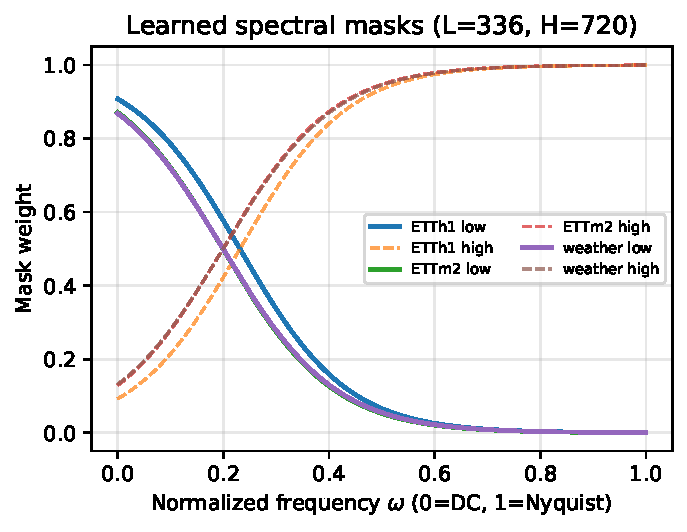
\includegraphics[width=0.82\linewidth]{../results/figures/learned_filter.pdf}%
  }{\fbox{\parbox[c][0.20\textheight][c]{0.8\linewidth}{\centering
    \textbf{[learned filter figure pending]}}}}
  \caption{Learned low/high spectral masks of \method's partition-of-unity
  decomposition as a function of normalized frequency.}
  \label{fig:learned_filter}
\end{figure}

\begin{figure}[t]
  \centering
  \IfFileExists{../results/figures/arevin_profile.pdf}{%
    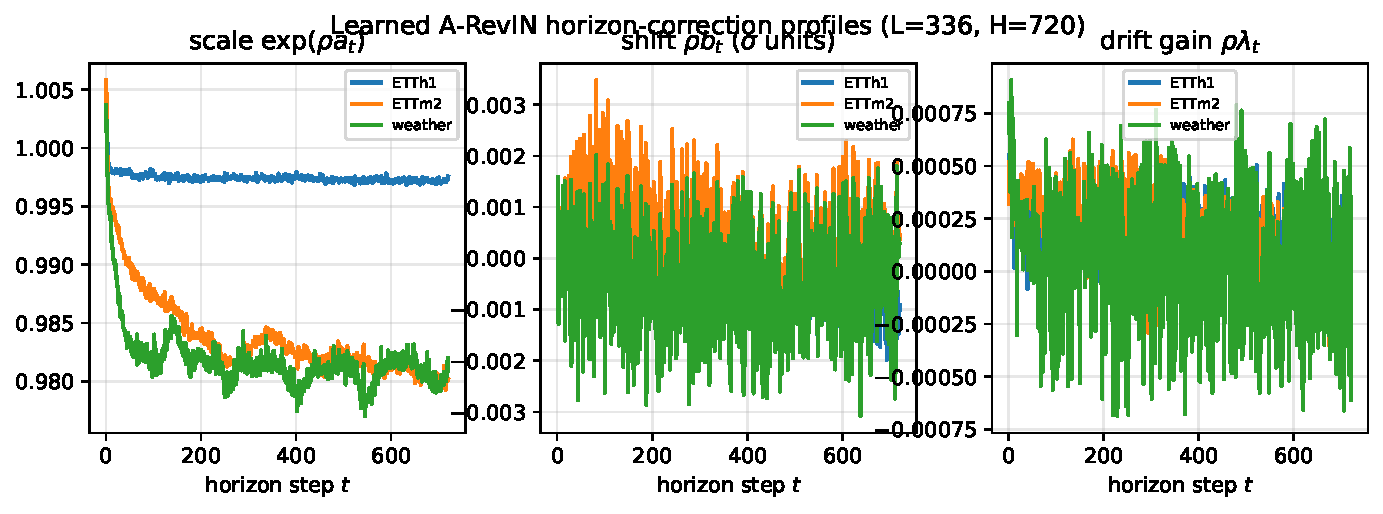
\includegraphics[width=0.82\linewidth]{../results/figures/arevin_profile.pdf}%
  }{\fbox{\parbox[c][0.20\textheight][c]{0.8\linewidth}{\centering
    \textbf{[A-RevIN profile figure pending]}}}}
  \caption{Per-step \arevin\ correction profile across the forecast horizon,
  showing how the adaptive de-normalization varies with horizon distance.}
  \label{fig:arevin_profile}
\end{figure}

\subsection{A Controlled Study: \arevin\ Engages with Non-stationarity}
\label{sec:results:synthetic}

The ILI result shows \arevin\ helping on a real strongly non-stationary dataset,
but real data confounds non-stationarity with many other factors. To confirm the
mechanism directly, we construct a synthetic benchmark in which the
non-stationarity magnitude is the \emph{only} thing that varies. Each series has
four channels and length $4000$ and is the sum of (i) a stationary seasonal base
with periods $24$ and $168$, (ii) Gaussian observation noise, and (iii)
$\delta$ times a unit-variance \emph{persistent} trend---an AR(1)-smoothed random
slope that is locally linear and therefore extrapolatable. The seasonal base and
the trend signal are \emph{shared} across all values of $\delta$, so increasing
$\delta$ injects more non-stationarity while holding everything else fixed; at
$\delta{=}0$ the series is stationary. We isolate \arevin\ by comparing RLinear
(plain RevIN) against an A-RevIN-Linear ($K{=}1$, identical backbone) at
$L{=}96, H{=}96$ over three seeds.

Table~\ref{tab:synthetic} reports the MSE reduction of \arevin\ over RevIN and the
learned mean gate $\bar\rho$ as $\delta$ increases. The benefit rises
\emph{monotonically} with injected drift---from neutral-to-slightly-negative when
the series is stationary or mildly non-stationary ($-0.28\%$ at $\delta{=}0$,
$-0.23\%$ at $\delta{=}0.5$, $-0.09\%$ at $\delta{=}1$) to a clear positive gain
as drift grows ($+0.30\%$ at $\delta{=}2$, $+1.42\%$ at $\delta{=}4$), with the
learned gate widening accordingly ($\bar\rho$ from $0.52$ to $0.54$). This is a
controlled confirmation of the mechanism that complements the ILI result: under
stationarity \arevin\ is harmless and reduces to RevIN, and its advantage grows
precisely with the non-stationarity it is designed to handle. As elsewhere, we
note honestly that the absolute gains are modest.

\IfFileExists{../results/tables/synthetic_table.tex}{%
\begin{table}[t]\centering
\caption{Controlled synthetic-drift study at $L{=}96, H{=}96$ (3 seeds). $\delta$
scales the injected persistent trend ($\delta{=}0$ is stationary). $\Delta\%$ is
the MSE reduction of A-RevIN-Linear over RLinear (plain RevIN) on the identical
backbone; $\bar\rho$ is \arevin's learned mean gate. The benefit increases
monotonically with $\delta$.}
\label{tab:synthetic}
\begin{tabular}{lrrrr}
\toprule
$\delta$ & RLinear & A-RevIN-Lin. & $\Delta$\% & learned $\bar\rho$ \\
\midrule
0 & 0.1150 & 0.1153 & -0.28 & 0.52 \\
0.5 & 0.1227 & 0.1230 & -0.23 & 0.52 \\
1 & 0.1348 & 0.1349 & -0.09 & 0.52 \\
2 & 0.1382 & 0.1378 & +0.30 & 0.52 \\
4 & 0.1097 & 0.1081 & +1.42 & 0.54 \\
\bottomrule
\end{tabular}
\end{table}}{\begin{table}[t]\centering\caption{Synthetic-drift study.}%
\label{tab:synthetic}\textit{[synthetic table pending]}\end{table}}

\begin{figure}[t]
  \centering
  \IfFileExists{../results/figures/synthetic_drift.pdf}{%
    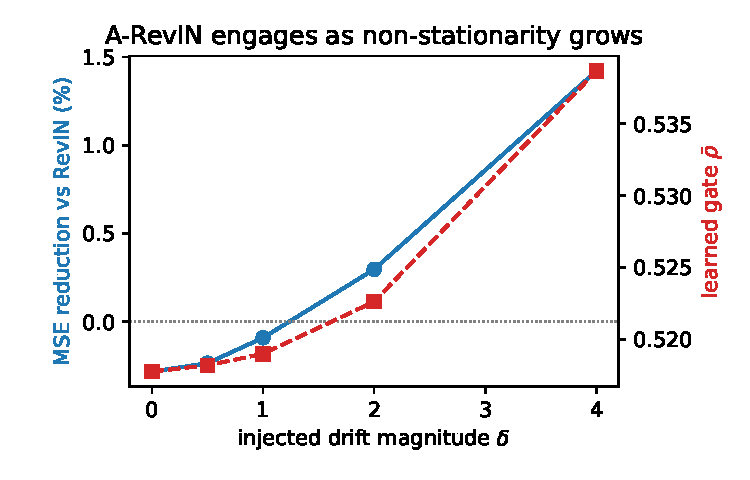
\includegraphics[width=0.82\linewidth]{../results/figures/synthetic_drift.pdf}%
  }{\fbox{\parbox[c][0.20\textheight][c]{0.8\linewidth}{\centering
    \textbf{[synthetic-drift figure pending]}}}}
  \caption{\arevin's benefit and its learned gate both increase with injected
  non-stationarity: MSE reduction over RevIN and learned mean gate $\bar\rho$ as
  functions of the controlled drift magnitude $\delta$.}
  \label{fig:synthetic}
\end{figure}
